\documentclass[11pt]{article}


\usepackage{amsmath}
\usepackage{amssymb}
\usepackage[utf8]{inputenc}
%\usepackage[latin1]{inputenc}
\usepackage[spanish]{babel}
\usepackage[left=3cm,right=3cm,top=3cm,bottom=2.5cm]{geometry}
\usepackage{amsmath,amssymb,latexsym,color,graphicx,verbatim}
\usepackage{mathrsfs}
\usepackage{layout}
\usepackage{graphicx}


%COLOCA COMANDOS EN ESPAÑOL
%\renewcommand{\contentsname}{Contenido}
%\renewcommand{\partname}{Parte}
%\renewcommand{\appendixname}{Apéndice}
%\renewcommand{\figurename}{Figura}
%\renewcommand{\tablename}{Tabla}
%\renewcommand{\abstractname}{Resumen}
%\renewcommand{\refname}{Bibliografía}
%FIN DEL BLOQUE
\usepackage[acronym,shortcuts]{glossaries} %PARA UN GLOSARIO DE ACRÓNIMOS
\makeglossaries
\usepackage[font=small]{caption}
\usepackage[colorlinks = true,
                     linkcolor = blue,
                     citecolor = red,
                     urlcolor = blue]{hyperref}

\baselineskip0.75cm
\parskip0.5cm
\parindent0cm

\begin{document}


\begin{titlepage}
\centering {\Large {\sc Calibración del espectrografo EShel- II PF0011}}

\vfill
\centering {\Large Propuesta de trabajo de grado para optar al t\'itulo de F\'isico}
\vfill
\hfill

\centering {\Large Jesús Alberto Sánchez Villafrades$^{1,2}$}

\vfill

\centering {\Large Director: Luis Alberto Núñez$^{1,2}$}

\centering {\Large Co-Director: $^{3}$}



\hfill






{{\Large $^1$Grupo de Investigaci\'on en Relatividad y Gravitaci\'on GIRG}} \\
{{\Large$^2$Grupo Halley de Astronom\'ia y Ciencias Aeroespaciales}} \\

\vfill
\vfill

\centering {\Large Universidad Industrial de Santander\\Facultad de
Ciencias\\Escuela de F\'{i}sica\\Bucaramanga\\2018}


\end{titlepage}


\newpage

\tableofcontents

%\newpage

%\acrodef{LAGO}{Latin American Giant Observatory}

\newpage


\begin{abstract}



 

%Surge entonces, la necesidad de mejorar las capacidades de la red de detección. En este trabajo se propone estudiar la pertinencia de la construcción y uso de perfiles atmosféricos mensuales, basados en datos extraídos del Global Data Assimilation System  (GDAS) para los sitios de LAGO. Así mismo, para verificar la efectividad de esta implementación los cálculos del flujo serán contrastados entre si.

\vspace{0.5cm}
Palabras clave: 

\end{abstract}




%%%%%%%%%%%%%%%%%%%%%%%%%%%%%%%%%%%%%%%%%%%%%%%%%%%%%%%%%%%%%%%%%%%%%%%%%%%%%%%%%%%%%%%%%%%%%%
\section{Introducci\'on}


%%%%%%%%%%%%%%%%%%%%%%%%%%%%%%%%%%%%%%%%%%%%%%%%%%%%%%%%%%%%%%%%%%%%%%%%%%%%%%%%%%%%%%%%%%%%%%








%%%%%%%%%%%%%%%%%%%%%%%%%%%%%%%%%%%%%%%%%%%%%%%%%%%%%%%%%%%%




\section{Marco teórico}
La espectroscopia estudia la interacción entre la radiación electromagnética y la materia,en astronomía esta radiación es emitida por estrellas y otros objetos celestes y al ser dispersada brinda mucha información de la fuente que la genero.\\
Para el caso del espectro visible esta Luz puede ser dispersada usando un prisma mediante el fenómeno de refracción o usando una rejilla de difracción, estos espectros dan información importante de las características físicas del objeto que las emite,están directamente relacionadas con la temperatura superficial del objeto así como con su composición química. Usando Efecto Dopler se puede tener información de la velocidad de rotación y traslación además de densidad y presión.
\cite{utilidad}\\

\subsection {Principios de la espectroscopia.}
Todo elemento que  irradie luz presenta en esta luz información detallada de las propiedades constituyentes de dicho elemento así como su temperatura, esta luz esta compuesta de múltiples longitudes de onda que son separadas y se pueden observar en un sensor ccd en forma de linea espectral, que es la distribución de  la intensidad en función de la longitud de onda o la frecuencia  de luz dispersada.

\subsection {Espectros y lineas espectrales.}

Históricamente las lineas espectrales fueron llamadas así ya que se  presenta como lineas de obscuridad o luminosidad en la salida de un espectroscopio luego de la dispersión, por esto la forma de las lineas dependen del instrumento que se este utilizando.\\
Estas lineas son de origen cuántico y se generan por la transición de 2 niveles de energía, estos puede dividirse en 3 tipos,las lineas espectrales continuas ,de emisión y las de absorción.\cite{troccoli}


\textbf{Espectro Continuo:}
Se define un espectro continuo cuando la franja de colores  pasa de un color a otro sin ninguna interrupción de franjas negras entra color y color como se presente en la figura 1, se puede observar esto con la luz blanca y en general cualquier solido o gas sometido a altas presiones o temperaturas presente un espectro continuo.


\begin{figure}[htb!]
\centering

\includegraphics[width=0.7\textwidth]{1}
\caption[Descripción versión comprimida]{Espectro continuo.\cite{libro}}
 \label{fig:fig6}
\end{figure}

\textbf{Espectro de emisión :} Un gas a baja presión y excitado a altas temperaturas produce un espectro de emisión,estos espectros constan de rayas de diversos colores separadas por amplias zonas  negras en las que no se observa luz ver figura 2. Este tipo de espectro se da cuando los electrones en los átomos de estos gases excitados absorben energía de la fuente que los esta excitando  y saltan a orbitas superiores , la emisión tiene lugar cuando los electrones caen a niveles mas bajos emitiendo este exceso de energía en forma de fotones con una frecuencia característica propia de cada elemento.


 \begin{figure}[htb!]
\centering
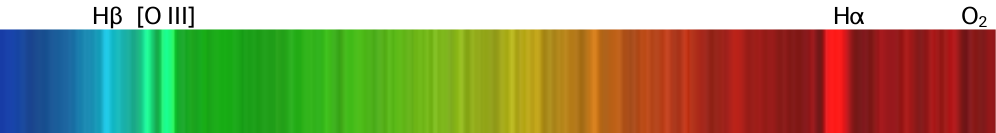
\includegraphics[width=0.7\textwidth]{2}
\caption[Descripción versión comprimida]{El espectro de emisión del hidrógeno \cite{articulo1}}
 \label{fig:fig6}
\end{figure}


\textbf{Espectro de absorción :} Este tipo de espectro se da cuando se hace pasar luz blanca a través de un gas frío a baja presión, el espectro que se observa presenta un fondo de color con franjas negras, con la característica principal de que las lineas de absorción aparecen en el mismo lugar que las lineas de emisión.\\
En astronomía las fuente luminosa generalmente es una estrella, la luz proveniente de la estrella atraviesa capas de gas propia de la atmósfera, las lineas de absorción dependerán estrictamente de la composición química del gas, esta absolverá fotones de una u otra longitud de onda dejando las franjas obscuras características de espectro de absorción.


\begin{figure}[htb!]
\centering
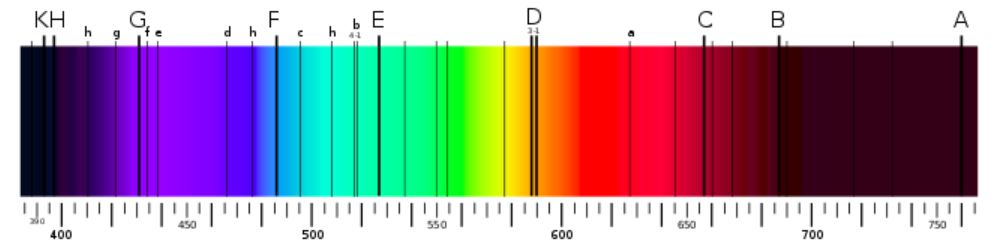
\includegraphics[width=0.7\textwidth]{3}
\caption[Descripción versión comprimida]{Espectro solar en el que se aprecian las líneas principales de von Fraunhofer. \cite{articulo1}}
 \label{fig:fig6}
\end{figure}

%falta citar de https://culturacientifica.com/2019/08/13/los-espectros-de-absorcion-de-los-gases/

Los anteriores espectros tienen su explicación en las leyes de kirchof  que se presentan a continuación.

-Un espectro continuo se produce por un un solido incandescente o un gas a alta presión.

-Un espectro de emisión se produce por un gas incandescente a baja presión.

- Cuando se hace pasar luz blanca a través de un gas a baja presión y baja temperatura se produce un espectro de emisión.

\subsection {Radiación de cuerpo negro}
Es bien conocido el fenómeno por el cual todos los cuerpos que se encuentran por encima del cero absoluto presentan radiación electromagnética, a altas temperaturas se habla de incandescencia pues las longitudes de onda de emisión se encuentran en el espectro visible (entre 400 y 700 nm) aun a bajas temperaturas  el objeto seguirá irradiando pero ahora en el infrarroja (longitudes de onda superiores a 700 nm).\cite{libro2} \\
Kirchoff propuso en 1860   una hipótesis  de radiación para los cuerpo en equilibrio , la denomino radiación de cuerpo negro, esta muestra como la radiación tiene un patrón regular que depende de la temperatura.Mas tarde  Wein y Plank  hicieron el desarrollo matemático e este fenómeno, que se puede modelar como:

\begin{center}
    \begin{equation}
        \lambda_{max}=\frac{0.002898}{T}
    \end{equation}{}
\end{center}{}

Donde $ \lambda$ es la longitud de onda máxima emitida por el cuerpo y T es la temperatura en grados Kelvin.

\textbf{Ley de desplazamiento de Wien:}Durante el año 1893 Wien basándose en argumentos estadístico dedujo que la distribución normal de radiación, como era conocida hasta la fecha se modelaba  con la expresión:  

\begin{center}
    \begin{equation}
        I(\nu,T)=\nu^3f\[\left(\frac{\nu}{T}\right)\]
    \end{equation}{}
\end{center}{}

Donde $f(\left\frac{\nu}{T}\right)$ es desconocida pero solo puede depender de $\nu$ y de T.\\
Sin embargo Wien usando los datos de los experimentos realizados en la época pudo llegar a una expresión mas detallada para la ecuación  (2).  








\begin{figure}[htb!]
\centering
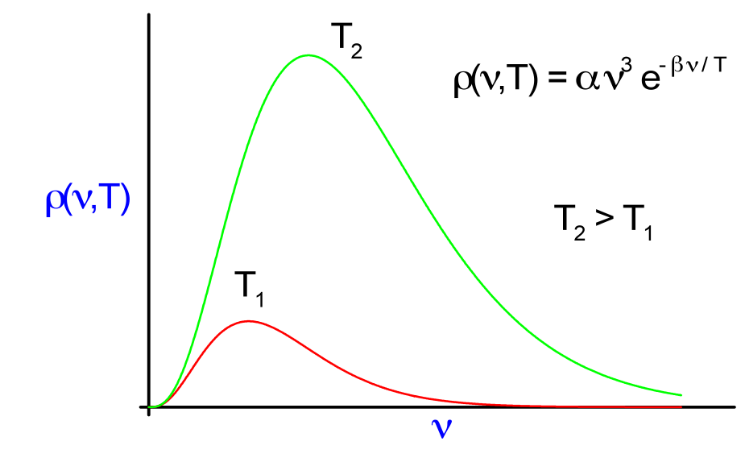
\includegraphics[width=0.6\textwidth]{5}
\caption[Descripción versión comprimida]{\cite{articulo1}}
 \label{fig:fig6}
\end{figure}











\subsection {Diagramas de Hertzsprung-Russell}



La espectroscopía permitiío la construccion del diagrama Hertzsprung-Russell, el cual se desarroll
o inicialmente en la Universidad de Harvard.
Este diagrama muestra la etapa de evolucion
de las estrellas con las lneas espectrales que se~nala el estado de los elementos qumicos presentes
en ellas. La figura 2.3 muestra como se relacionan las estrellas en tama~no, color, luminosidad,
clase espectral y la magnitud absoluta. Cada punto en este diagrama representa una
estrella en el rmamento, cuya magnitud y clase espectral absoluta han sido determinadas.
Los datos se agrupan en: estrellas de secuencia principal, supergigantes, gigantes y enanas
blancas.



%\subsection {Lineas de franhofer}








%%%%%%%%%%%%%%%%%%%%%%%%%%%%%%%%%%%%%%%



%%%%%%%%%%%%%%%%%%%%%%%%%%%%%%%%%%%%%%%%%%%%%%%%%%%%%%%%%%%%%%%%%%%%%%%%%%%%%%%%%%%%%%%%%%%%%%
\section{Objetivos}

%%%%%%%%%%%%%%%%%%%%%%%%%%%%%%%%%%%%%%%%%%%%%%%%%%%%%%%%%%%%%%%%%%%%%%%%%%%%%%%%%%%%%%%%%%%%%

\begin{itemize}
\item \textbf{Objetivo General}

Realizar el montaje, calibración y puesta en funcionamiento de ESPECTROGRAFO eShel II con el que cuenta el Grupo Halley de Astronoḿıa y Ciencias Aeroespacialesde la Universidad Industrial de Santander.\\

\item \textbf{Objetivos Espec\'ificos}
\end{itemize}

\begin{itemize}


\item Verificar el enfoque del lente colimador del espectrógrafo eShel II verificándolos con lineas de lamparas de emisión.

\item Realizar la calibración pixel-Longitud de onda mediante el software IRAF, usando lamparas de calibración con espectros conocidos.

\item Realizar los cálculos de la masa de aire para la ciudad de Bucaramanga de forma teórica.

\end{itemize}
%%%%%%%%%%%%%%%%%%%%%%%%%%%%%%%%%%%%%%%%%%%%%%%%%%%%%%%%%%%%%%%%%%%%%%%%%%%%%%%%%%%%%%%%%%%%%%




\newpage

%%%%%%%%%%%%%%%%%%%%%%%%%%%%%%%%%%%%%%%%%%%%%%%%%%%%%%%%%%%%%%%%%%%%%%%%%%%%%%%%%%%%%%%%%%%%%%
%%%%%%%%%%%%%%%%%%%%%%%%%%%%%%%%%%%%%%%%%%%%%%%%%%%%%%%%%%%%%%%%%%%%%%%%%%%%%%%%%%%%%%%%%%%%%%
\section{Metodolog\'ia}

El telescopio CDK 17 (corrected Dall-kirkham) es un telescopio de tubo ópticoo de diseño abierto, hecho en fibra de carbono con un paso de 43 kg, cuenta con 2 lentes de 90 mm (aplanadores de campo) y 2 espejos. 
Un espejo primario elipsoidal con una apertura de 432 mm y una relación focal de f/2,6 y un espejo secundario con una apertura de 159 mm con forma esférica.\\
Posee un enfocador Hedrik 3.5 y tres ventiladores en la parte inferior y 4 en las laterales del tubo óptico, todo esto acoplado a una montura ecuatorial Paramount ME II.\\
La montura Paramout ME II tiene un eje de contrapeso DEC 47 CM  de largo y 48 mm de diametro, 2 contrapesos de 14 Kg, un rodamiento de declinacion de 48 puntos de contacto, con una capacidad de carga de 140 Kg.






Para cumplir con los objetivos planteados se llevara la siguiente metodología.

\begin{itemize}

\item[1] Montaje del espectrógrafo con sus respectivo modulo de calibración y acople al telescopio.

\item[2] hacer el calculo de forma experimental de la rendija del espejo que permite el paso de luz al espectrógrafo.

\item[3] Realizar la captura de imágenes limpias de diferentes lamparas de emisión de laboratorio con el fin de garantizar que los elementos dispersores del espectrógrafo estén alineados con la cámara y se puedan reproducir espectros conocidos.

\item[3] Se calibrara la Montura robotizada PARAMOUNT  usando el software T-Point para garantizar un correcto apunte del telescopio al objeto de interés.



 
\end{itemize}

%%%%%%%%%%%%%%%%%%%%%%%%%%%%%%%%%%%%%%%%%%%%%%%%%%%%%%%%%%%%%%%%%%%%%%%%%%%%%%%%%%%%%%%%%%%%%%


%%%%%%%%%%%%%%%%%%%%%%%%%%%%%%%%%%%%%%%%%%%%%%%%%%%%%%%%%%%%%%%%%%%%%%%%%%%%%%%%%%%%%%%%%%%%%%
\section{Cronograma de Actividades}	
%%%%%%%%%%%%%%%%%%%%%%%%%%%%%%%%%%%%%%%%%%%%%%%%%%%%%%%%%%%%%%%%%%%%%%%%%%%%%%%%%%%%%%%%%%%%%%


\begin{center}
{\small
\begin{tabular}{|c|c|c|c|c|c|c|c|}
\hline

\textbf{Mes}/\textbf{Actividad}&\textbf{Act 1.1}&\textbf{Act 1.2}
&\textbf{Act 1.3}&\textbf{Act 2}&\textbf{Act 3}&\textbf{Act 4}&\textbf{Act 5}\\

\hline

Enero&$\bigotimes$&&&&&&\\

\hline

Febrero&$\bigotimes$&$\bigotimes$&&&&&\\

\hline

Marzo&&$\bigotimes$&$\bigotimes$&&&&\\

\hline

Abril&&&$\bigotimes$&&&&\\

\hline

Mayo&&&$\bigotimes$&$\bigotimes$&&&\\

\hline

Junio&&&$\bigotimes$&$\bigotimes$&&&\\

\hline
Julio&&&$\bigotimes$&$\bigotimes$&$\bigotimes$&&$\bigotimes$\\

\hline

Agosto&&&&&$\bigotimes$&$\bigotimes$&\\

\hline 

Septiembre&&&&&&&$\bigotimes$\\

\hline
Octubre&&&&&&&$\bigotimes$\\
\hline

\end{tabular}
}
\end{center}



%%%%%%%%%%%%%%%%%%%%%%%%%%%%%%%%%%%%%%%%%%%%%%%%%%%%%%%%%%%%%%%%%%%%%%%%%%%%%%%%%%%%%%%%%%%%%%
\medskip
\bibliographystyle{unsrt}
\bibliography{Tesis.bib}





%%%%%%%%%%%%%%%%%%%%%%%%%%%%%%%%%%%%%%%%%%%%%%%%%%%%%%%%%%%%%%%%%%%%%%%%%%%%%%%%%%%%%%%%%%%%%%
\end{document}
Al hacer las primeras aproximaciones de 

